\documentclass[11pt,notitlepage]{article}
\usepackage[english]{babel}
\usepackage{graphicx}
\usepackage{amsfonts}
\usepackage{amsmath}
\usepackage{ mathdots }

\usepackage{amsthm}
\usepackage{enumitem}
\usepackage[font=small, format=hang]{caption}
\numberwithin{equation}{section}


\usepackage[retainorgcmds]{IEEEtrantools}
%\usepackage{bbold}

\usepackage{indentfirst}
\usepackage{color}

\usepackage{changepage}
\usepackage{fullpage}

\usepackage{lipsum}

%---------------------------------------------------------------------------------------------
%               MACROS
%---------------------------------------------------------------------------------------------

%-----TO DO---------------
\newcommand{\todo}[1]{\marginpar[\textcolor{red}{TODO: #1}]{\textcolor{red}{TODO: #1}}
	\PackageWarning{TODO:}{#1!}}

%------Vectors style--------
\renewcommand{\vec}[1]{\mathbf{#1}}

%-----VECTORS COMMANDS-------
\def\R{{\mathbb{R}}}
\def\Rn{{\mathbb{R}^n}}
\def\K{{\mathbb{K}}}
\newcommand{\seg}[2]{{[\vec{0},\vec{#1}_{#2}]}}
\def\veconeton{{\{\vec{v}_1,\ \ldots\ , \vec{v}_n\}}}
\def\ei{{\vec{e}_i}}
\def\ej{{\vec{e}_j}}
\def\el{{\vec{e}_l}}
\def\vi{{\vec{v}_i}}
\def\vip{{\vi'}}
\def\vj{{\vec{v}_j}}
\def\vjp{{\vj'}}
\def\tr{{\,\!^t}}
\newcommand{\proj}[2][H^k]{{#2 \mid #1}}
%\def\ones{{\mathbb{1}}
%\def\onesv{{\vec{\ones}}

%------LOGIC CONNECTORS--------
\def\iff{{\Leftrightarrow}}
\def\then{{\Rightarrow}}
%\defcmd{{\Leftarrow}

%------CONVERGENCE--------
\def\normdist{\mathcal{N}}
\def\asconv{\stackrel{\text{a.s.}}{\longrightarrow}}

%------OPERATORS----------
\def\sumin{{\sum_{i=1}^{n}}}
\def\sumjn{{\sum_{j=1}^{n}}}
\def\ca{{c_\alpha}}
\def\sa{{s_\alpha}}
\def\nchoosek{{\binom{[n]}{k}}}

\DeclareMathOperator{\NTK}{NTK}
\DeclareMathOperator{\CNTK}{CNTK}
\DeclareMathOperator{\rank}{rank}
\DeclareMathOperator{\poly}{poly}

%\newcounter{definitions}
%\newcounter{thms}
%\newcounter{lemmas}


\newtheorem{theorem}{Theorem}[section]
\newtheorem{lemma}[theorem]{Lemma}
\newtheorem{corollary}{Corollary}[theorem]

\theoremstyle{remark}
\newtheorem*{rmk}{Remark}

\theoremstyle{definition}
\newtheorem{definition_body}[theorem]{Definition}
\newtheorem*{notation_body}{Notation}

\renewenvironment{proof}[1][\proofname]{{\bfseries #1.\linebreak}}{\qed\\
	
	} %To make "Proof" BOLD

%-----DEFINITIONS----------
\newcommand{\definition}[1]{
	\theoremstyle{definition}
	\begin{definition_body}
		#1
	\end{definition_body}
	\theoremstyle{plain}
}

%------NOTATION----------
\newcommand{\notation}[1]{
	\theoremstyle{definition}
	\begin{notation_body}
		#1
	\end{notation_body}
	\theoremstyle{plain}
}

%------REMARKS----------
\newcommand{\remark}[1]{
	\theoremstyle{remark}
	\begin{rmk}
		#1
	\end{rmk}
	\theoremstyle{plain}
}

%---------------------------------------------------------------------------------------------
%               END
%---------------------------------------------------------------------------------------------


\title{Convolutional Neural Tangent Kernel}
\author{William Cappelletti}
\date{\today}

\begin{document}
	\begin{titlepage}
		\centering
		\vspace*{0.cm}
		{\Huge \textsc{Convolutional Neural Tangent Kernel\\}}
		\vspace*{0.3cm}
		\textbf{---}\\
		\vspace*{0.3cm}
		{\Large \textsc{William Cappelletti\\}}
		\vspace*{0.7cm}
		
		\begin{abstract}
			In this paper, we study the relation between artificial neural networks and kernel regression.
			We start by defining some neural networks, such as the multilayer perceptron (MLP) and the convolutional neural network (CNN); then we discuss some theoretical results that support the equivalence with kernel methods.			
			We use \emph{tensor programs} to see that at initialization infinitely wide neural networks are equivalent to Gaussian processes.
			Then, we study the \emph{Neural Tangent Kernel}, which gives the direction along which the network evolves during training.
			In the infinite width limit of MLPs, this kernel converges to a finite one and is constant during training.
			Furthermore, if the MLP is big enough, with high probability, the function given by the network after training is close to the function given by the kernel regressor using the limiting Neural Tangent Kernel.
			
			At this point, we test the kernel regressor against the actual neural network.
			We do so with a multilayer perceptron and a convolutional neural network, which we train and test on the MNIST handwritten digits dataset, on a classification task.
		\end{abstract}
		
		
		\vspace*{1cm}
		{\large \textbf{Semester Project\\
				\vspace*{0.1cm}
				under the supervision of\\
				Professor C. Hongler and Dr. F. Gabriel}\\}
		\vspace*{0.2cm}
		SFL Chair\\
		\vspace*{1cm}
		\textbf{Autumn 2019}\\
%		\vspace*{0.6cm}
		\begin{figure}[h]
			\begin{center}
				\includegraphics[width=8cm]{../../../epfl.png}
			\end{center}
		\end{figure}
		Mathematics Section\\
		MSc in Applied Mathematics 2019--2020
		
		
	
	\end{titlepage}
	\pagenumbering{gobble}% Remove page numbers (and reset to 1)
	
	\tableofcontents		
	
	\newpage
	\pagenumbering{arabic}
	    
	\section{Introduction}\label{sec:Introduction}
	In this paper we study the relation between artificial neural networks and kernel regression.
	We start by defining some neural networks, such as the multilayer perceptron and the convolutional neural network; then we discuss some theoretical results that support the relation with kernel methods.
	
	It has been proved, in \cite{neal2012bayesian}, \cite{jacot2018neural}, and \cite{yang2019scaling}, that at initialization, if the parameters are sampled independently at random with proper distribution, infinitely wide neural networks are equivalent to Gaussian processes.
	To understand what an infinitely wide network is and to justify this result, we report Yang definition of \emph{tensor programs}, \cite{yang2019scaling}, in Section \ref{subsec:tensorProg}.
	
	Then, in Section \ref{subsec:iwl}, we explain what it means for a network to be infinitely wide.
	Once this concept is clear, we give the conditions under which the infinite network behaves like a Gaussian process, which are quite general conditions satisfied by most standard deep learning architectures.
	
	We then follow \cite{jacot2018neural} and \cite{arora2019exact} and in Section \ref{subsec:ntk} we study the Neural Tangent Kernel, which gives the direction along which the network evolves during training.
	In \cite{jacot2018neural}, Jacot et al. proved that in the infinite width limit this kernel converges to a finite one and is constant during training.
	Then, in \cite{arora2019exact}, Arora et al. prove that if a network is big enough, with high probability, the function given by the network after training is close to the function given by the kernel regressor using the limiting Neural Tangent Kernel.
	
	At this point, we focus on the experimental part.
	Firstly, in Section \ref{sec:implementation}, we precise how to compute, practically, the Neural Tangent Kernel, with the technical limitations deriving from its definition.
	Then, in Section \ref{sec:experiments}, we test the kernel regressor against the actual neural network.
	We do so with a multilayer perceptron and a convolutional neural network, which we train and test on the MNIST handwritten digits dataset, on a classification task.
	The task consisting in recognising the digit drawn on a $28 \times 28$ grayscale image.
	
	We see that the kernel methods accuracy is worse than the actual neural network, but it is consistently close to it.
	
	
	\section{Artificial Neural Networks}
	Artificial Neural Networks (ANNs) describe a wide family of parametrized functions, which has gained more and more popularity thanks to their outstanding performances in various regression and classification tasks, as well as in computer vision and natural language processing, \cite{fleuret2019deep}.
	Many different structures exist and have different properties, but the main idea is that we model a function through many layers, composed by different nodes.
	Each node is a function of other nodes appearing in previous layers; more precisely, we take a linear combination of said nodes and then apply a nonlinear function to the output.
	
	The models are trained starting from a loss function, which gives a measure of the error with respect to the task the ANN should perform.
	We use this loss function to perform gradient descent, or variants of it, over the parameters of the network, using a technique known as backpropagation.
	
	To get a better understanding of this family of functions, we give two examples, which are widely used in practice, namely the multilayer perceptron and the convolutional neural network.
	We will focus on these two architectures for the experimental part.
	
	\subsection{Multilayer perceptron}
	The multilayer perceptron (MLP), also known as fully connected neural network, is the simplest example of ANN.
	It consists of an input layer and an arbitrary number, say $L$, of hidden layers, the last of which is also called the readout layer.
	The input layer is just the datapoint $x = x^{(0)} \in \R^{n^0} = \R^{n_{\text{in}}}$ that we feed into the network, where each coordinate is considired as a node.
	Each hidden layer $l$ consists of a weight matrix $w^{(l)} \in \R^{n^{l-1} \times n^l}$, a bias vector $b^{(l)} \in \R^{n^l}$ and a nonlinearity $\sigma$ which is applied component-wise.
	The nodes in the hidden layer $l$ corresponds to the values of the vector $x^{(l)}$ defined recursively as
	\begin{equation}
	x^{(l)} = \sigma(w^{(l)} \cdot x^{(l-1)} + b^{(l)}), \quad \forall l = 1, \dots, L.
	\end{equation}
	The readout layer describes a function of both the input and the parameters, namely $f(x;$ $w^{(1)}$, $b^{(1)}, \dots, w^{(L)}, b^{(L)})$.
	Figure \ref{fig:fullyConnected} illustrates an MLP with three hidden layers.
	
	\begin{figure}
		\centering
		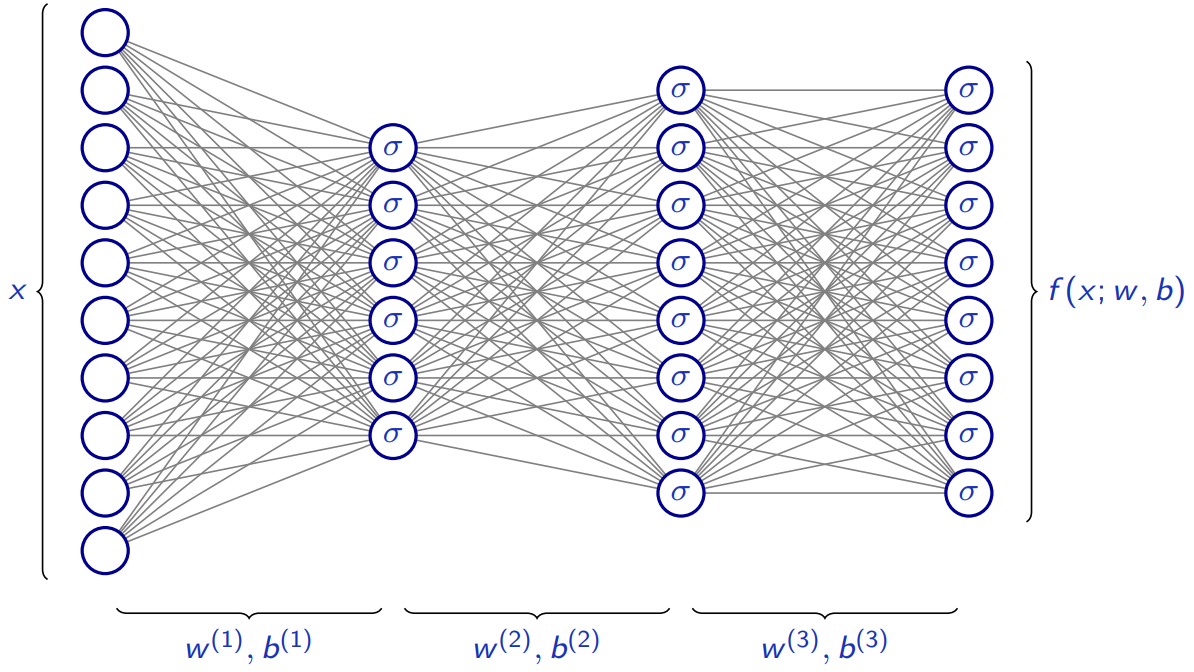
\includegraphics[width=.75\linewidth]{Figures/fully_connected.png}
		\caption{Illustration of a Multilayer perceptron with three hidden layers, from \cite{fleuret2019deep}.
			The last one, on the furthest right, is the readout layer $f(x; w, b)$, which is a function of both the input and the parameters.}
		\label{fig:fullyConnected}
	\end{figure}
	
	\subsection{Convolutional Neural Network}
	Convolutional neural networks (CNNs) are generally used with image inputs, i.e. two or three-dimensional tensor.
	They work by concatenating different convolutional layers, which are, basically, filters on images.
	
	We can imagine a grayscale picture as a matrix encoding each pixel luminosity, which is a two-dimensional tensor, having a \emph{width} and a \emph{heigth}; on the other hand, colour images are encoded as three matrices, each one encoding the luminosity of a different primary colour (for instance Red, Green and Blue).
	In the latter case, we can stack the three matrices in one three dimensional tensor, the third dimension being referred to as \emph{channel}.
	
	What a convolutional layer does, in practice, is applying a filter, across multiple channels to parts of the images in a convolutional way, hence the name.
	To give a precise definition, we let $P$ be the width and $Q$ be the height of the image, in practice $P=Q$.
	We use $q \times q' \in \mathbb{N} \times \mathbb{N}$ to denote the filter size.
	For a convolutional filter $w \in  \R^{q \times q' }$ and an image $x \in \R^{P \times Q} $, the convolution operator is defined as
	\begin{equation}\label{eq:convolution}
	[w * x]_{ij} = \sum_{a=1}^{q} \sum_{b=1}^{q'}
	[w]_{a, b}[x]_{a+i, b+j}, \quad \text{for } i\in [P - q + 1], j \in [Q - q' + 1].
	\end{equation}
	
	The CNN is then defined recursively as follows
	\begin{itemize}
		\item Let $x^{(0)} = x \in R^{P \times Q \times C^(0)}$ be the input image, where $C^{(0)}$ is the initial number of channels.
		\item For $h = 1, \dots , L,$ $\beta = 1, \dots , C^{(h)}$, the intermediate outputs are defined as
		\begin{equation}\label{eq:convolutionalLayer}
		x_{(\beta)}^{(h)} = \sigma\left(\sum_{\alpha=1}^{C^{(h-1)}} W^{(h)}_{(\alpha), (\beta)} * x^{(h-1)}_{(\alpha)}\right),
		\end{equation}
		where each $W^{(h)}_{(\alpha), (\beta)}$ is a filter with appropriate size and $\sigma$ is a nonlinear function applied component-wise.
	\end{itemize}
	As we can see from \eqref{eq:convolutionalLayer}, the number of channels changes from one layer to the other (from $C^{(h-1)}$ to $C^{(h)}$) and from \eqref{eq:convolution} the image size shrinks according to the filter size (as the filter cannot move outside the boundaries of previous layer).
	Figure \ref{fig:convolution} illustration of a convolutional layer.
	
	\begin{figure}
		\centering
		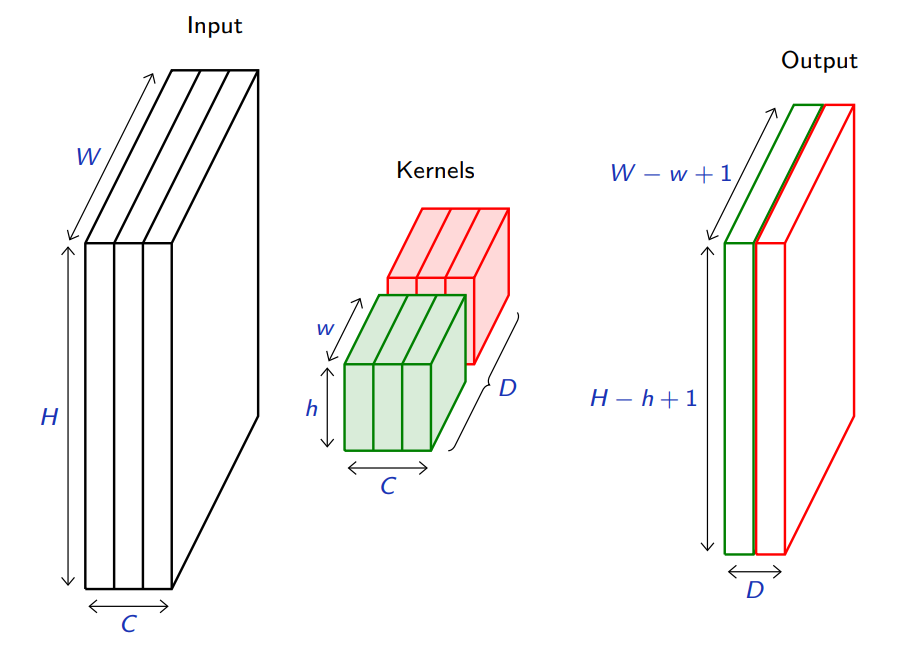
\includegraphics[width=.5\linewidth]{Figures/convolution.png}
		\caption{Illustration of a convolutional layer, from \cite{fleuret2019deep}. Kernel is used here as synonim for filter. $W$, $H$ and $C$ are width, height and number of channes of the input image; $w,h$ are width and height of the filters, $D$ is the number of channels of the output image.}
		\label{fig:convolution}
	\end{figure}
	\section{Neural Networks as Gaussian Processes}\label{sec:nnAsGaussianPr}
	
	\subsection{Tensor Programs}\label{subsec:tensorProg}
	
	Our goal is to study how Artificial Neural Networks (ANN) behaves when their sizes become arbitrarily big and their parameters are initialized at random, following Glorot initialization \cite{glorot2010understanding}.
	
	To study such functions, Yang introduces the concept of \emph{tensor program} in \cite{yang2019scaling} and \cite{yang2019tensor}.
	This framework is used to bind the sizes of parameters across different parts of the network, by explicitly binding to a line of the program introduction and usage of each parameter and non-linearity.
	
	\definition{
		We consider programs of the following form, which we call \emph{tensor programs}. Each line $l$ contains an assignment and a dimension annotation and can have the following types.
		\begin{itemize}
			\item \textbf{VecIn} (G) a vector input $x$
			\[l: g^l := x \in \R^{n^l}; \]
			\item \textbf{MatIN} (A) a matrix input $A$
			\[l: A^l := A \in\R^{n^l_1 \times n^l_2}; \]
			\item \textbf{T} (A) transpose of an A-var
			\[l: A^l := (A^j)^\tr \in \R^{n^l_1 \times n^l_2} = \R^{n^j_2 \times n^j_1}; \]
			\item \textbf{MatMul} (G) if $A^k$ and $g^j$ have $n^k_2 = n^j$, then an assignement via a linear mapping
			\[l: g^l := A^kg^j \in \R^{n^l} = \R^{n_1^k}; \]
			or similarly for H-vars
			\[l: g^l := A^kh^j \in \R^{n^l} = \R^{n^k_1} \] where $j,k < l$;
			\item \textbf{LinComb} (G) if $n^{j_1} = \dots = n^{j_k}$, then an assignment via linear combination of G-vars that apperared in previous lines: with $a^l_{j_i} \in \R$,
			\[l: g^l := a^l_{j_1}g^{j_1} + \cdots + a^l_{j_k}g^{j_k} \in \R^{n^{j_1}}; \]
			\item \textbf{Nonlin} (H) if $n^{j_1} = \dots = n^j_k$, then an assignement via some general (possibly nonlinear) function $\phi^l : \R^k \rightarrow \R$, acting coordinatewise,
			\[l: h^l := \phi^l( g^{j_1}, \dots, g^{j_k}) \in \R^{n^l} = \R^{n^{j_1}}. \]
		\end{itemize}
		
		The letters in parentheses indicate a naming convention for the variables introduced in each line and group them according to similar properties.
		We call \emph{G-vars} the assignments of VecIn, MatMul and LinComb; \emph{A-vars} those of MatIn and T; and \emph{H-vars} the variables assigned by Nonlin.
		
	}
	
	In short, \emph{tensor programs} allow the input of vectors (\textbf{VecIn}) and matrices (\textbf{MatIn}) and their usage in linear combination of vectors (\textbf{LinComb}), matrix multiplication (\textbf{MatMul}), matrix transpose (\textbf{T}) and application of general (possibly nonlinear) functions (\textbf{Nonlin}).
	Some examples of standard deep learning architectures, translated as tensor programs, can be found in \cite[Section 3]{yang2019scaling} and, in fact, this convention can express almost any neural network.
	In spite of being more cumbersome of the usual algebraic formulation, this notation makes it easier to study ANN as we let their sizes increase arbitrarily.
	
	Intuitively, each program line $l$ binds a variable assignment ($g^l$, $A^l$ or $h^l$) and a dimension annotation ($n^l$ or $n^l_1 \times n^l_2$), such that one can use each line result in other operations and keep track of the relations between dimensions.
	It follows that lines of type T, MatMul, LinComb, and Nonlin induce equality constraints on the dimensions of each line.
	
	Given a program $\pi$ and a possible set of additional dimensional constraints $\Lambda$, we can consider the smallest equivalence relation $\sim$ on G-vars such that $g \sim g'$ if their dimensions are constrained to be equal by $\Lambda$ or by some line of the program.
	With this relation, we can split the G-vars into classes and we call each class a \emph{common dimension class} (CDC); we write $\mathfrak{C}$ the collection of all CDCs for a program $\pi$ and additional constraints $\Lambda$.
	The CDCs are the main instrument to understand the ANN behaviour when we let the network's dimensions increase, as all its elements scale together.
	
	\subsection{The Infinite Width Limit}\label{subsec:iwl}
	
	We study how ANNs behave when we let their dimensions go to infinity, in what is called the Infinite Width Limit.
	Before we go deeper into theoretical results, we want to clarify what it means, for different architectures, to become infinitely wide.
	The easiest case is the multilayer perceptron (MLP), which is a simple neural network in which all layers are fully connected.
	By definition, the only dimensions that are bound are the input size of a layer and the output size of the previous one.
	Therefore, each layer gives its own CDC and the dimensions that go to infinity are the number of nodes in each layer (i.e the columns in each weight matrix and bias vector).
	This justifies the approach used in \cite{jacot2018neural}, where the authors make layers sizes increase to infinity sequentially.
	
	A different intuition arises when considering CNNs.
	In this case, by the definition of convolution, one cannot have the size of the filter to grow to infinity, as that would impose all layers to grow to infinity together and it would require an infinite size input, which is absurd.
	Therefore, in such a situation, the filter size stays the same, and the dimension that grows to infinity, in each layer, is the number of channels.
	To visualize what that means in terms of tensor programs, we can consider an image with different channels.
	We take a vector across channels for every single pixel and we can see each filter application as first multiplying each pixel-vector by a weight matrix, giving as result a pixel-vector with a different number of channels, and then obtaining the preactivations for each coordinate of the new tensor as linear combinations of the latter pixel-vectors.
	Finally, one can apply the nonlinearity pointwise.
	For a complete example, we refer the reader to \cite[Appendix B.6]{yang2019scaling}.
	
	In the same way, we can express through tensor programs more complex architectures, such as Residual Neural Networks and other kinds of transformer, as shown in \cite[Appendix B]{yang2019scaling}.
	After we understand what dimensions go to infinity, we can prove that some similar behaviour arises, in spite of the architectures being significantly different.
	The first consequence is that in the \emph{Infinite Width Limit} all ANNs behave like \emph{Gaussian Processes}.
	
	Neal first proved, in \cite{neal2012bayesian}, that a single-layer neural network with random parameters can converge in distribution to a Gaussian process as its width goes to infinity. In \cite{yang2019scaling}, Yang extends this result to any network that can be described by a tensor program.
	
	We consider a sequence (in $t \in \mathbb{N}$) of dimensions $\{n^{lt}\}_{g^l \text{ or } h^l} \cup \{n_1^{lt}, n_2^{lt}\}_{A^l}$ respecting the equivalence relation $\sim$ (defined in Section \ref{subsec:tensorProg}) in the program $\pi$, where $g^l$, $h^l$ and $A^l$ are, respectively, G, H, and A-vars appearing at line $l$ in $\pi$.
	At time $t$, we sample independently $A^{lt}_{ij} \sim \normdist(0, (\sigma^{lt})^2/n_2^{lt})$, for each $i$, $j$, for a set $\{\sigma^{lt} \}_{A^l}$ (this is the well established Glorot initialization).
	For each common dimension class $\mathfrak{c}$, we also sample independenty $g^{\mathfrak{c}_{\text{in}}t} \sim \normdist(\mu^{\mathfrak{c}_{\text{in}}t}, K^{\mathfrak{c}_{\text{in}}t})$ for each $i$.
	Here $\mathfrak{c}_{\text{in}}$ is the set of input G-vars in $\mathfrak{c}$, $g^{\mathfrak{c}_{\text{in}}t} = (g^{lt}_i)_{g^l \in \mathfrak{c}_{\text{in}}}$, and $\mu^{\mathfrak{c}_{\text{in}}t}: \mathfrak{c}_{\text{in}} \rightarrow \R, K^{\mathfrak{c}_{\text{in}}t}: \mathfrak{c}_{\text{in}} \times \mathfrak{c}_{\text{in}} \rightarrow \R$ are specified mean and covariance at time $t$.
	Thus, given $(\pi, \Lambda)$, the data $\{n^{\mathfrak{c}t}\}_{\mathfrak{c} \in \mathfrak{C}}$, $\{\sigma^{lt}\}_{A^l}$, $\{\mu^{\mathfrak{c}_{\text{in}}t}\}_{\mathfrak{c} \in \mathfrak{C}}$ and $\{K^{\mathfrak{c}_{\text{in}}t}\}_{\mathfrak{c} \in \mathfrak{C}}$ realize a random program $\pi(\{n^{\mathfrak{c}t}\}_{\mathfrak{c} \in \mathfrak{C}}, \{\sigma^{lt}\}_{A^l}, \{\mu^{\mathfrak{c}_{\text{in}}t}\}_{\mathfrak{c} \in \mathfrak{C}}, \{K^{\mathfrak{c}_{\text{in}}t}\}_{\mathfrak{c} \in \mathfrak{C}})$.
	
	Furthermore, we assume that as $t \rightarrow \infty$, for all $\mathfrak{c}$, $\mathfrak{c}' \in \mathfrak{C}$:
	\begin{enumerate}[itemsep=0em, topsep=3pt]
		\item $n^{\mathfrak{c}t}$ is increasing with $t$ and $n^{\mathfrak{c}t} \rightarrow \infty$.
		\item $\lim_{t \rightarrow \infty} n^{\mathfrak{c}t} / n^{\mathfrak{c}'t} = \alpha_{\mathfrak{c}, \mathfrak{c}'} \in (0, \infty)$, for some constant $\alpha_{\mathfrak{c}, \mathfrak{c}'}$ depending only on $\mathfrak{c}' \in \mathfrak{C}$.
		\item $\sigma^{lt} \rightarrow \sigma^{l\infty}$ for some finite $\sigma^{l\infty} > 0$ for each input A-var $A^l$.
		\item $\mu^{\mathfrak{c}_{\text{in}}t} \rightarrow \mu^{\mathfrak{c}_{\text{in}}\infty}$ and $K^{\mathfrak{c}_{\text{in}}t} \rightarrow K^{\mathfrak{c}_{\text{in}}\infty}$ for some finite $\mu^{\mathfrak{c}_{\text{in}}\infty}$ and $K^{\mathfrak{c}_{\text{in}}\infty}$, and $\rank K^{\mathfrak{c}_{\text{in}}t} = \rank K^{\mathfrak{c}_{\text{in}}\infty}$ for all large $t$.
	\end{enumerate}
	
	Finally, for the main theorem proved by Yang in \cite{yang2019scaling} to hold, we need to restrict to a general class of nonlinearities, which we can intuitively think as meaning that the function is at most exponential.
	
	\definition{
		For $\alpha > 0$, a function $\phi : \R^k \rightarrow \R$ is said to be \emph{$alpha$-controlled} if for some $C$, $c > 0$, we have
		\begin{equation}
		|\phi(x)| \leq \exp\left(C \sum_{i=1}^k|x_i|^\alpha + c \right)
		\end{equation}
		for all $x \in \R^k$.
	}
	
	\begin{theorem}[G. Yang 2019, \cite{yang2019scaling} and \cite{yang2019tensor}]\label{thm:yangMaster}
		Consider dimension constraints $\Lambda$ and a program $\pi$ without T lines, i.e. no transpose allowed. Suppose the nonlinearities are $\alpha$-controlled for some $\alpha <2$. Sample all input vars as explained beforehand (Glorot initialization). Then, for any $\mathfrak{c} \in \mathfrak{C}$ and any $\alpha$-controlled function $\psi : \R^{\mathfrak{c}} \rightarrow \R$, $\alpha < 2$,
		\begin{equation}
		\frac{1}{n^{\mathfrak{c}t}}\sum_{i=1}^{n^{\mathfrak{c}t}} \psi (g_i^{\mathfrak{c}t}) 
		\asconv \mathbb{E}\psi(Z),
		\end{equation}
		where $g^{\mathfrak{c}t}_i = (g^{lt}_i)_{g^l \in \mathfrak{c}}$ and $\R^{\mathfrak{c}} \ni Z = (Z^g)_{g \in \mathfrak{c}} \sim \normdist(\mu^{\mathfrak{c}}, K^{\mathfrak{c}})$, with $\mu^{\mathfrak{c}}$ and $K^{\mathfrak{c}}$ defined respectively in \eqref{eq:mean} and \eqref{eq:covariance}.
	\end{theorem}
	
	For any $\mathfrak{c} \in \mathfrak{C}$, we recursively define
	\begin{equation}\label{eq:mean}
	\text{(mean)} \quad \mu^{\mathfrak{c}}(g^l) =
	\begin{cases}
	\mu^{\mathfrak{c}_{\text{in}}\infty}(g^l) & \text{if } g^l \in \mathfrak{c}_{\text{in}}\\
	\sum_i a^l_{ji} \mu^{\mathfrak{c}}(g^j_i) & \text{if } g^l := \sum_i a^l_{ji} g^j_i \\
	0 & \text{if } g^l := A^k g^j \text{ or } g^l := A^k h^j
	\end{cases}
	\end{equation}
	and recursively define
	\begin{equation}\label{eq:covariance}
	\text{(covariance)} \quad K^{\mathfrak{c}}(g^l, g^m) =
	\begin{cases}
	K^{\mathfrak{c}_{\text{in}}\infty}(g^l, g^m) & \text{if } g^l, g^m \in \mathfrak{c}_{\text{in}}\\
	\sum_i a^m_{ji} K^{\mathfrak{c}}(g^l, g^j_i) & \text{if } g^m := \sum_i a^m_{ji} g^j_i \\
	\sum_i a^l_{ji} K^{\mathfrak{c}}(g^j_i, g^m) & \text{if } g^l := \sum_i a^l_{ji} g^j_i \\
	(\sigma^{k\infty})^2 \mathbb{E}_z[\phi^a(z)\phi^b(z)] & \text{if } g^l:= A^k h^a, g^m := A^k h^b \\
	0 & \text{else}
	\end{cases}
	\end{equation}
	where $h^a := \phi^a(g^j_1, \dots, g^j_k), h^b := \phi^b(g^{j'}_1, \dots, g^{j'}_k)$ and $z \sim \normdist(\mu^{\mathfrak{c}}, K^{\mathfrak{c}})$.
	Note that \eqref{eq:mean} and \eqref{eq:covariance} keep track of how the mean and covariance change while the variables pass through the network. The different branches characterize which kind of tensor program line assigned the variables $g^l$ and $g^m$.
	
	We now make a more technical comment about the recursion.
	While other branches are more clear, note that branch 4 in \eqref{eq:covariance} also covers the case when $g^l := A^k g^a$ or $g^m := A^k g^b$ by ``typecasting'' $g^a$ to an H-var and setting $\phi^a$ = id (similarly for $g^b$).
	Finally, remark that $\phi^a$ will ignore irrelevant components of a, and the expectations only depend on the entries of $\mu^{\mathfrak{c}}$ and $K^{\mathfrak{c}}$ that correspond to already-defined values, so this describes a valid recursion.
	
	\begin{figure}[h!]
		\centering
		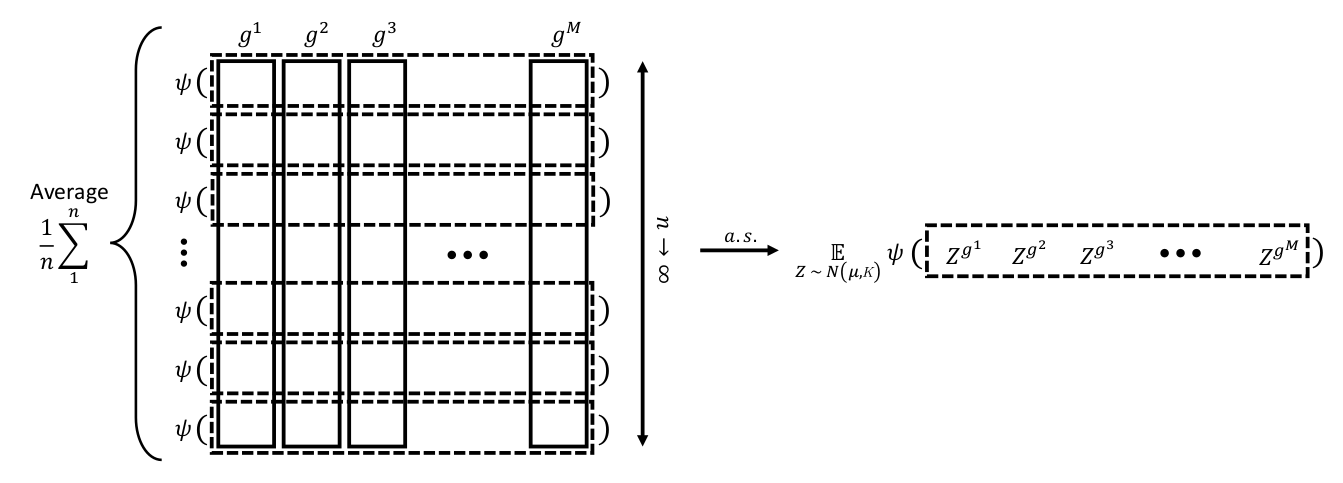
\includegraphics[width=\linewidth]{Figures/NETSOR_master_thm1.png}
		\caption{Illustration of Theorem \ref{thm:yangMaster}, from \cite{yang2019tensor}. If we suppose that $g^1, \dots, g^M$ are all the G-vars in a CDC (i.e. $g^{\mathfrak{c}} = (g^1, \dots, g^M)$), then, as the dimension $n$ increase, the empirical mean along the coordinates of the G-vars of an $\alpha$-controlled function $\psi$ converges to the expected value.
			Or, more intuitively, for each $i$, $(g^1_i, \dots, g^M_i) \approx \normdist(\mu, K)$.
		}
	\end{figure} 
	
	Intuitively, Theorem \ref{thm:yangMaster} states that $g_i^{\mathfrak{c}t} \stackrel{\text{d}}{\approx} \normdist(\mu^\mathfrak{c}, K^\mathfrak{c})$ for large $t$, iid for each $i$.
	This, jointly with the definitions of \eqref{eq:mean} and \eqref{eq:covariance}, means, roughly speaking, that the G-vars (preactivations, CFR Section \ref{subsec:tensorProg}) created from the same matrix $A^k$ have nonzero correlations, but otherwise are asymptotically independent unless they appear together in a LinComb.
	The latter can be seen by checking which entries of $K^\mathfrak{c}$ are nonzero by \eqref{eq:covariance}, in fact, the only nonzero values are those corresponding to the first four branches, which characterize G-vars that are either correlated by initialization (first branch), or if at some point they pass through the same matrix $A^k$ (fourth branch), as the second and third, being recursive, will at some point lead to one of those cases.
	
	\subsection{Neural Tangent Kernel}\label{subsec:ntk}
	
	Has we have seen in Section \ref{subsec:iwl}, each neural network architecture is equivalent, in the infinite width limit to a Gaussian Process.
	This implies that we can study the regression we perform with the ANN as a kernel method, once we understand which kernel corresponds to its training.
	In this section, $\{x^i\}_{i\in [N]} \subset \R^{\text{dim}_\text{in}}$ denote the network inputs, $\theta \in \R^P$ contains all the parameters, distributed at initialization as in Section \ref{subsec:iwl}, and $f(\theta, x)$ is the output of the network, which, for notation simplicity, we suppose unidimensional in this section.
	
	As in \cite{jacot2018neural} and \cite{arora2019exact}, we consider a training dataset $\{(x^i, y^i)\}_{i=1}^N \subset \R^{d_\text{in}} \times \R$ and we train the neural network by minimizing a convex loss function \[l(\theta) = \sum_{i=1}^N\mathcal{L}(f(\theta, x^i), y^i). \]
	We update the parameters at step $t$ using gradient descent with an infinitesimally small learning rate $\frac{d\theta(t)}{dt} = - \nabla l(\theta(t))$.
	With this setup, if we consider $l$ to be the mean squared error, by a simple differentiation \cite[Lemma 3.1]{arora2019exact} we see that the outputs of the network $u(t) = (f(\theta(t), x^i))_{i\in [N]}$ evolve according to 
	\begin{equation}\label{eq:dynamics}
	\frac{du(t)}{dt} = -\NTK(f_t) \cdot (u(t) - y),
	\end{equation}
	where $\NTK(f_t)$ is the $n \times n$ positive semidefinite matrix given by the \emph{Neural Tangent Kernel}.
	
	\definition{
		With the notation previously introduced, we define the \emph{Neural Tangent Kernel} $\NTK(\cdot, \cdot)$ as the kernel whose values on points $x, x'$ are given by 
		\begin{equation}\label{eq:ntk}
		\NTK(x, x') = \left\langle \frac{\partial f (\theta, x)}{\partial \theta}, \frac{\partial f (\theta, x')}{\partial \theta} \right\rangle. 
		\end{equation}
		
		For any kernel $K$, we abuse the notation and, when the context make it clear, use $K$, or specifically $NTK$, to define the matrix whose entries $i,j$ are given by $K(x^i,x^j)$.
	}
	
	As we can see, the $\NTK$ depends on the parameters of the network and thus it is random at initialization and varies during training.
	Nonetheless, as NTK is an $\alpha$-controlled function on the inputs $x, x'$, if we let the network go to the infinite width limit, as explained in Section \ref{subsec:iwl}, we can apply Theorem \ref{thm:yangMaster} and see that the tangent kernel converges to a finite limit, as proved in \cite{jacot2018neural} and \cite{yang2019scaling}.
	
	\definition{We denote this limiting kernel $\NTK_\infty$.}
	
	Going back to the dynamic expressed in \eqref{eq:dynamics}, we see that if the network is infinitely wide, the expression is identical to that of \emph{kernel regression} under gradient flow, as $\NTK(f_t) = \NTK_\infty$ is constant during training, \cite{jacot2018neural}.
	
	Although we started by considering only the mean squared error loss, it turns out that this idea applies to a wide variety of cases.
	In fact, in \cite{jacot2018neural}, Jacot et al. prove that the network function of an MLP evolves along the kernel gradient given by the Neural Tangent Kernel for any convex loss function.
	We conjecture that this result holds for any deep learning architecture.
	
	\subsection{Kernel Regression}\label{subsec:kernelRegression}
	
	Before moving to the experimental part, we remind the reader some concepts about \emph{kernel regression}.
	Suppose we have a kernel function $K(\cdot, \cdot)$ and a training dataset $\{(x^i, y^i)\}_{i=1}^N \subset \R^{d_\text{in}} \times \R$, kernel regression aims to approximate the underlying function with the linear combination
	\begin{equation}\label{eq:kernelReg}
	f_K(\cdot) = \sum_{i=1}^N \alpha^i K(\cdot, x^i).
	\end{equation}
	
	The coefficients are estimated to minimize the loss function over prediction points
	\begin{equation*}
	l(\alpha) = \mathcal{L}(f(x_*), y_*),
	\end{equation*}
	and, in practice, this minimization is carried over the training dataset
	\begin{equation}\label{eq:kernelCoeff}
	\widehat{\alpha} = \arg\inf\left\{\sum_{i=1}^N \mathcal{L}\left(\sum_{j=1}^N \alpha_j K(x^i,x^j), y^i\right) : \alpha_1,\dots, \alpha_N \in \R \right\}.
	\end{equation}
	
	There is a nontrivial result linking a fully trained wide MLP $f_{nn}$ to the kernel regression predictor $f_{\NTK}$, using the $\NTK_\infty$.
	If we consider a fresh observation $x^*$ and let $f_{nn} := \lim_{t \rightarrow \infty} f(\theta(t), x^*)$, where $f(\theta(t), \cdot)$ is the MLP output function as in Section \ref{subsec:ntk}, we can prove the following theorem.
	\begin{theorem}[Arora et al. 2019, \cite{arora2019exact}]
		Suppose an MLP with ReLU activation function and $L$ hidden layers with $m$ nodes, whwre $m \geq \poly(1/\kappa, L, 1/\lambda_0, N, \log(1/\delta))$, $N$ being the size of the training dataset, $1/\kappa = \poly(1/\epsilon, \log(n/\delta))$ and $\lambda_0$ being the smallest eigenvalue of the matrix $NTK_\infty$ over the training data.
		Then, for any $x^* \in \R^{d_\text{in}}$ with $||x^*|| = 1$, with probability at least $1-\delta$ over the random initialization, we have 
		\[|f_{nn}(x^*) - f_{\NTK}(x^*)| \leq \epsilon. \]
	\end{theorem}
	The main consequence of this theorem is that, if a network is big enough, then we can expect its performace to be similar to that of the NTK regressor, with a non-asymptotic bound.
	
	\subsection{Multidimensional output}
	
	All we stated before about neural networks and kernels generalize immediately to the multi\-dimensional case upon noting that a function $f : \R^{d_\text{in}} \rightarrow \R^{d_\text{out}}$ is equivalent to a function $\tilde{f} : \R^{d_\text{in}} \times [d_\text{out}] \rightarrow \R$ with $\tilde{f}(x, k) = f_k(x)$.
	This said we can generalize kernel regression, with each entry of the kernel $K(x, x')$ now being a matrix instead of a scalar and $\alpha$ being a vector, such that the vector-matrix product in \eqref{eq:kernelReg} produces indeed a vector output.
	In this case, the kernel matrix $K$ is a block matrix, where each block is given by the matrix $K(x^i, x^j)$.
	
	For the Neural Tangent Kernel, this means that 
	\begin{equation}\label{eq:multiNtk}
	[NTK(x^i,x^j)]_{k, k'} = \left\langle \frac{\partial f_k (\theta, x^i)}{\partial \theta}, \frac{\partial f_{k'} (\theta, x^j)}{\partial \theta} \right\rangle,
	\end{equation}
	with $k,k' \in [d_\text{out}]$.
	An interesting point of the multidimensional approach is that, as we can see in \eqref{eq:multiNtk}, the kernel also encodes information between different output coordinates, i.e. $k \neq k'$.
	
	%    \section{Asymptotics results}\label{sec:asympthotics}
	
	\section{NTK implementation}\label{sec:implementation}
	
	To practically test the theoretical results on different deep learning architectures, we choose to work using the efficient and popular library \verb|Pytorch| \cite{pytorch}, which is highly optimized for tensorial calculus.
	We gave in \eqref{eq:ntk} an explicit formula to compute the NTK of a given neural network.
	This formulation is very suitable for the \verb|Autograd| functionality of \verb|Pytorch|.
	In fact, this module creates a computational graph when input is passed through the ANN and it is then possible to quickly compute derivatives with respect to the network parameters.
	
	\subsection{NTK for finite networks}\label{subsec:finiteImpl}
	To get the exact NTK corresponding to a finite network, we choose therefore to compute the full Jacobian \verb|Jac| of the function $f(\theta, (x^1, \dots, x^N))$, where we pass all the input variables in a batch.
	In this way, we get a tensor of size $N \times d_\text{out} \times P$, where $N$ is the number of data points, $d_\text{out}$ is the length of the response vector and $P$ is the number of parameters in the network, i.e. the length of $\theta$.
	At this point, we can compute the kernel by multiplying the Jacobian by its transpose (as it is a tensor we intend the transpose along the two fist axes, corresponding to the input number and the coordinate of the output layer) and then by adding up the entries over the third ax, namely the one corresponding to parameters.
	This last step cab be written in one line using Einstein summation convention, and computed efficiently in \verb|Pytorch| with the function \verb|einsum| and then reshaping the matrix:
	\begin{verbatim}
	einsum('abp, cdp -> abcd', Jac, Jac).reshape(N * dim_out, N * dim_out)
	\end{verbatim}
	
	There are two main limitations to this approach.
	First of all, the Jacobian requires a lot of memory to be stored.
	For instance, if we consider an MLP with 3 hidden layers, 100 nodes in each layer and output size of 10, with biases at each layer; and we want to use it for a handwritten digit classification, for which the standard input images have $28 \times 28$ grayscale pixels, our network would have $99710 \approx 10^5$ parameters.
	This, jointly with a $1000$ regression images, would require a tensor of size $10^3 \times 10 \times 10^5$, thus with a billion entries.
	Supposing we store each digit at 32-bit precision, the Jacobian would require approximately $3$GB of memory.
	Then, another Jacobian would be necessary for prediction, thus doubling the memory required, if we suppose the test set to have equal size as the training one.
	
	Secondly, as a consequence of \verb|Pythorch| differentiation implementation, to retrieve the full Jacobian we need to iterate both on input images and on output dimensions.
	This is because differentiation always return a tensor of the same shape as the variable by which we differentiate and, thus, in case the derivative is a tensor of higher dimension, requires a direction over which aggregate the derivatives, which in this case would be a matrix with rows correspond to images and columns to output coordinates.
	This double loop seriously affects computation time, as the very fast \verb|Pythorch| backend is accessed without any optimization through the \verb|python| loops, which are very slow as it is an interpreted language.
	
	\subsection{NTK at infinite width}\label{subsec:infinteImpl}
	To estimate $\NTK_\infty$, i.e. the kernel corresponding to the ANN in the infinite width limit, we have different options.
	The first one would be to find an explicit formula and exactly compute the kernel function, as Arora et al. did in \cite{arora2019exact}.
	Although explicit formulas are already known for MLPs and elementary CNNs, to compute them still requires to go through all layers, all input images and all output dimensions, which implies more and more computations the deeper the network is.
	Furthermore, every different architecture would explicitly require an explicit formula, which should be obtained beforehand.
	
	We can avoid the latter problem leveraging on the fact that in the infinite width limit if our conjecture is right, each layer of the network has a kernel, which converges to the theoretical limiting one.
	We could thus use the already cited results, and iteratively compute an estimator of the kernel by passing through layers.
	By using the fact that, asymptotically, the kernel for each node is independent from the others, at least for MLPs \cite{jacot2018neural}, we can average of them to get an estimate of the actual value.
	Nonetheless, when considering more elaborate architectures, such as CNN or transformers, obtaining the NTK is not as straightforward.
	
	For this reason, we choose to follow the same approach as for the finite case.
	More precisely, we initialize many big networks, compute the NTK for each of them and then estimate the limiting kernel as their average.
	
	\section{Experimental results}\label{sec:experiments}
	
	In this section we focus on testing experimentally our conjecture, namely that all the results presented in Section \ref{sec:nnAsGaussianPr} generalize to general Deep Learning architectures as well.
	In particular, it has already been tested that for MLPs with a single output, regression based on NTK obtains results equivalent, or even better, than those of the original network.
	On the other hand, the same does not holds for CNNs, where experimental results show that the actual network greatly outperform the kernel methods \cite{arora2019exact}.
	Our objective is to understand what the network is actually learning, to confront it with what the $\NTK_\infty$ regression function, furthermore we study networks with multidimensional output.
	
	More precisely, given an ANN with random initialization, we can compute its actual $\NTK$, as explained in Section \ref{subsec:finiteImpl}, and its theoretical-infinite-wide counterpart $NTK_\infty$.
	Then, we train the ANN to get $f_{nn}$, which produces another tangent kernel $\NTK_{tr}$.
	By \cite{jacot2018neural}, we know that $NTK_\infty$ does not change during training, so we can study the kernel regression functions $f_{\NTK_\infty}$ and $f_{\NTK_{tr}}$ given respectively by the infinite width Tangent Kernel and the NTK obtained by the finite and trained Network.
	
	\subsection{The dataset}\label{subsec:dataset}
	
	\begin{figure}[t]
		\centering
		
\includegraphics[width=.75\linewidth]{../Simulations/figures/mnist_sample.png}
		\caption{Sample of 8 images from the MNIST dataset.
			The grayscale pictures represent, in the order, the digits 5, 0, 7, 1, 6, 9, 0, 7.}
	\end{figure}
	
	We perform an handwritten-digit classification task, using the MNIST dataset \cite{lecun2010mnist}.
	It consists in grayscale images of handwritten digits, whose size is 28x28 pixels, and their labels, which correspond to the 10 digits from 0 to 9.    
	We use 500 samples for train and we study the Kernel on a test of 500 samples.
	The two sets are disjoint and randomly drawn from the full dataset, using \verb|Pytorch| functionalities.
	
	We normalize the images beforehand, as the mean and standard deviation are well known, so that the observation space is supported in the unit sphere, which is one of the hypothesis used by Jacot et al. in \cite{jacot2018neural}.
	
	To train the ANNs and the coefficients for kernel regression we use the Cross entropy loss, which is the standard when performing a classification task.
	To optimize the parameters we use \verb|Adam| optimizer \cite{kingma2014adam} over 5000 epochs.
	
	\subsection{Multilayer Perceptron}
	
	We start with the artificial neural network on which all theoretical results have been proved.
	In particular, we test an architecture with three fully-connected hidden layers and a readout layer.
	The input dimension is of $784 = 28 \cdot 28$ nodes and all hidden layers have the same number of nodes.
	Combined with the readout layer, this gives a total of 99710 parameters.
	
	We proceed as explained beforehand.
	We estimate the limiting NTK at initialization on a big network with 200 nodes.
	Then we initialize an MLP with the same architecture but only 100 nodes and train it as explained beforehand.
	Computing the tangent kernel of the latter gives us two different kernels $\NTK_\infty$ and $\NTK_{tr}$, whose first entries we illustrate in Figure \ref{fig:ntk_before_after_tr}.
	\begin{figure}
		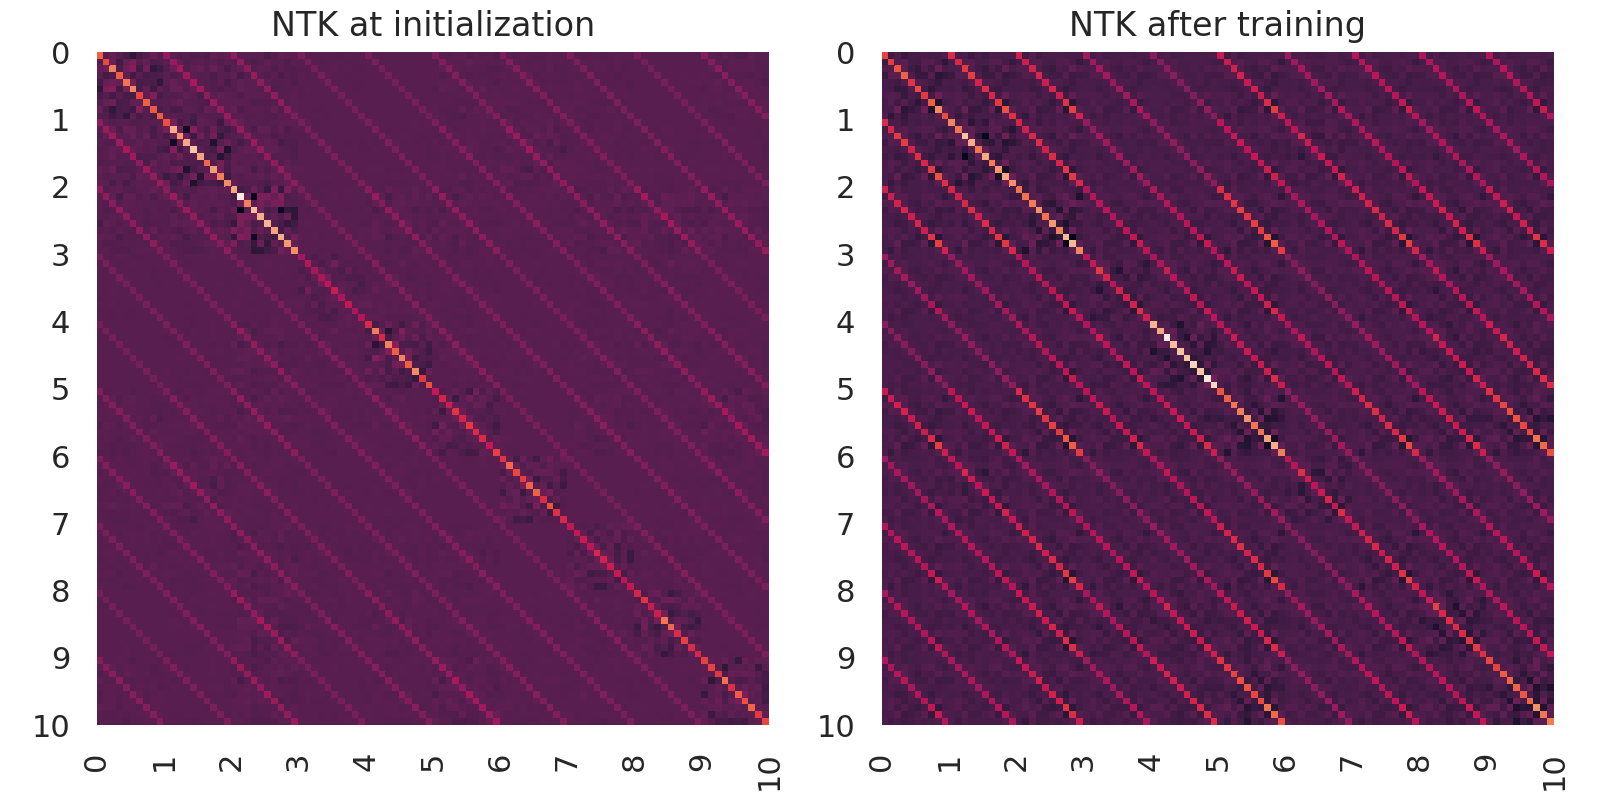
\includegraphics[width=\linewidth]{../Simulations/figures/ntk_before_after_tr.png}
		\caption{Neural Tangent Kernel of the MLP at initialization (Left) and after fully training the network (Right).
			The plot shows the entries of the first $10 \times 10$ blocks of the neural tangent kernel.
			Recall that each block represent $\NTK(x, x')$ and it is a $10 \times 10$ matrix, whose entries $k,l$ correspond to the scalar product of the gradients of $f_k$ and $f_l$ with respect to the model parameters. 
			Both images use a colour code to visualize the matrix and represent values close to zero in dark purple, but they have different scales.
			In fact, white values on the left are close to 24, while on the right they are close to 24000.
			This shows that the kernel does indeed move during training in the finite case.}
		\label{fig:ntk_before_after_tr}        
	\end{figure}
	
	We see that with 100 nodes the kernel still moves consistently during training.
	We then test if this change affects the performance of Kernel regression.
	As we did with the ANN, we train the coefficients of the two kernel regressor, $f_{\NTK_\infty}$ and $f_{\NTK_{tr}}$.
	Table \ref{tab:ntkScores} reports the results for the classification task.
	We see that on training all regressors perfectly fit the data, while the accuracy on test differs.
	In particular, none of the kernel regressors performs as well as the actual network, even though the kernel of the trained, smaller, network is closer to the expected result than $\NTK_\infty$.
	
	\begin{table}[th!]
		\centering
		\begin{tabular}{l|r|r}
			& Test accuracy & Train accuracy\\
			\hline
			MLP & 0.844 & 1.0 \\
			$\NTK_\infty$ & 0.73 & 1.0 \\
			$\NTK_{tr}$ & 0.804 & 1.0
		\end{tabular}
		\caption{Accuracy scores for the handwritten-digit recognition task. MLP is the fully trained multilayer perceptron, while $\NTK_\infty$ and $\NTK_{tr}$ refers to the two kernel regressors using the respective kernels.}
		\label{tab:ntkScores}
	\end{table}
	
	\subsection{Convolutional Neural Network}
	
	We now test the theoretical results on a convolutional neural network.
	In particular, we define an architecture with three convolutional layers, the first two with filters of size $5\times 5$ and the last one with a filter of size $20 \times 20$, so that the output will be a tensor of size $1 \times 1 \times 10$, each channel corresponding to the prediction for the corresponding digit.
	Again, the input dimension is a tensor of size $28 \times 28 \times 1$ and the number of channels passes from 1 to 15, to 15 and finally to 10.
	All the weights and biases considered, we have a total of 90550 parameters.
	
	We proceed as in previous section, but this time, for computational limitation, we use the same dimensions for both the network estimating the $\CNTK_\infty$ and that which we train.
	Again, we end up with two different kernels $\CNTK_\infty$ and $\CNTK_{tr}$, whose first entries we illustrate in Figure \ref{fig:cntk_before_after_tr}.
	\begin{figure}
		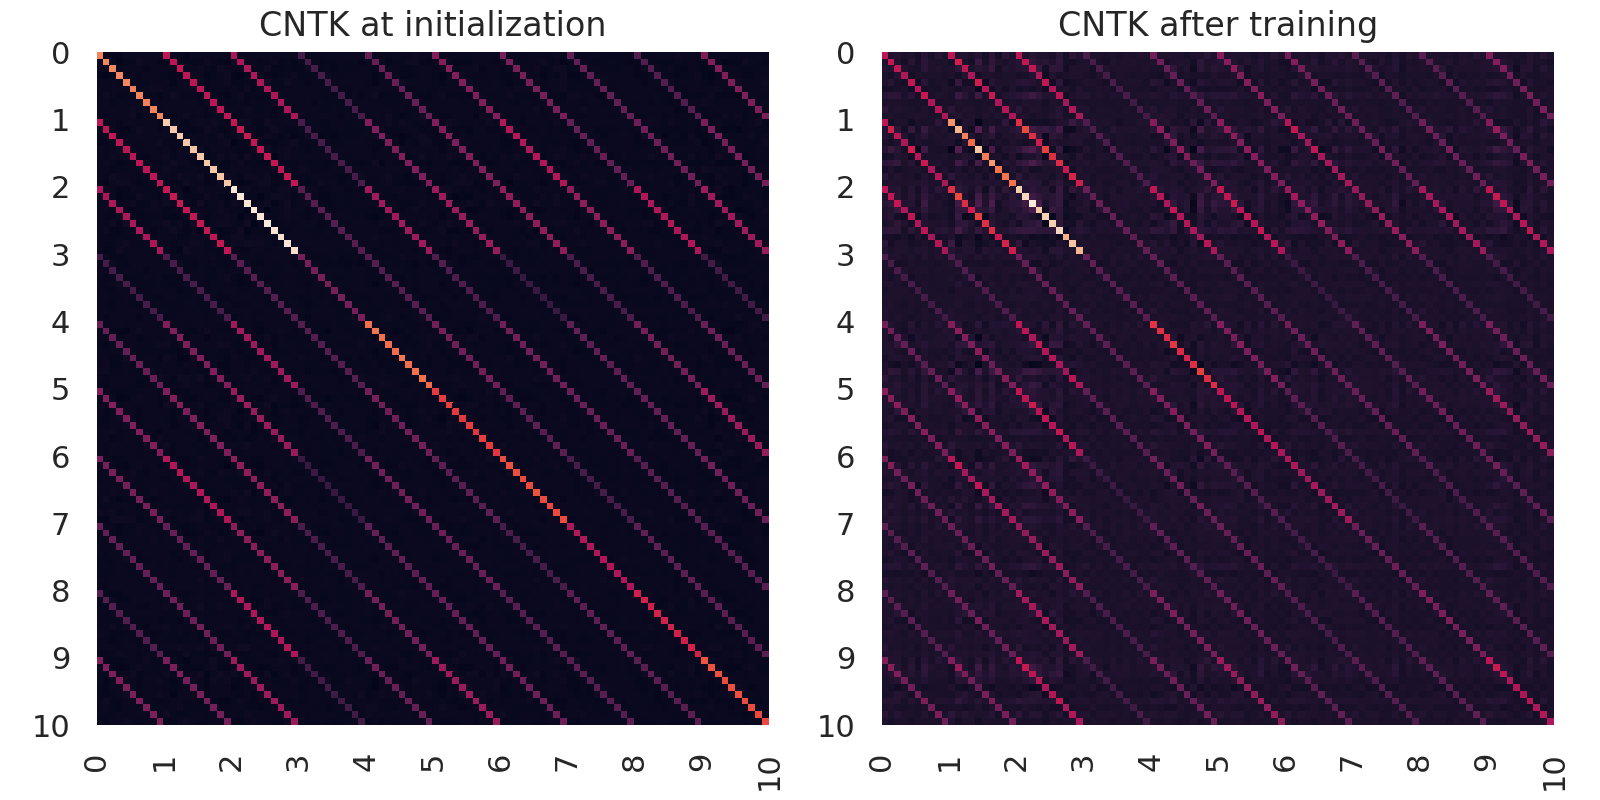
\includegraphics[width=\linewidth]{../Simulations/figures/cntk_before_after_tr.png}
		\caption{Convolutional Neural Tangent Kernel at initialization (Left) and after fully training the CNN (Right).
			The plot shows the entries of the first $10 \times 10$ blocks of the neural tangent kernel.
			Recall that each block represent $\CNTK(x, x')$ and it is a $10 \times 10$ matrix, whose entries $k,l$ correspond to the scalar product of the gradients of $f_k$ and $f_l$ with respect to the model parameters. 
			Both images use a colour code to visualize the matrix and represent values close to zero in dark purple, but they have different scales.
			In fact, white values on the left are close to 300, while on the right they are close to $10^5$.
			This shows that the kernel does indeed move during training in the finite case.}
		\label{fig:cntk_before_after_tr}        
	\end{figure}
	
	We see that with this setup the kernel still moves during training.
	It is interesting to note that the magnitude of the entries increases notably, as for the MLP, but the structure of the matrix, in terms of which values are close to zero and which are far from it, remains very similar.
	
	As before, we study how this change affects the performance of Kernel regression.
	We train the coefficients of the two kernel regressor, $f_{\CNTK_\infty}$ and $f_{\CNTK_{tr}}$ and
	Table \ref{tab:cntkScores} reports the results for the classification task.
	We see that on training the network and the trained kernel perfectly fit the data, while the regressor using $\CNTK_\infty$ does not fully train with 5000 epochs.
	As for the MLP case, the accuracies on the test set differ.
	Even though all performances are better than the MLP-related ones, none of the kernel regressors performs as well as the actual network.
	Nonetheless, it is notable that the differences presented are of the same order as before, with the initialization kernel scoring $10\%$ worse than the actual network and $5\%$ worse than the kernel obtained after training.
	
	\begin{table}[th!]
		\centering
		\begin{tabular}{l|r|r}
			& Test accuracy & Train accuracy\\
			\hline
			CNN & 0.894 & 1.0 \\
			$\CNTK_\infty$ & 0.802 & 0.928 \\
			$\CNTK_{tr}$ & 0.84 & 1.0
		\end{tabular}
		\caption{Accuracy scores for the handwritten-digit recognition task. MLP is the fully trained multilayer perceptron, while $\CNTK_\infty$ and $\CNTK_{tr}$ refers to the two kernel regressors using the respective kernels.}
		\label{tab:cntkScores}
	\end{table}

%	\begin{figure}[h]
%		\begin{minipage}{0.5\textwidth}
%			\centering
%			\includegraphics[height=0.6\textwidth,width=0.75\textwidth]{example-image-a}
%		\end{minipage}
%		\begin{minipage}{0.5\textwidth}
%			\centering
%			\includegraphics[height=0.6\textwidth,width=0.75\textwidth]{example-image-a}
%		\end{minipage}
%		\begin{minipage}{0.5\textwidth}
%		\begin{minipage}{0.5\textwidth}
%			\centering
%			\includegraphics[height=0.6\textwidth,width=0.75\textwidth]{example-image-a}
%		\end{minipage}
%		\captionof{figure}{Example of two \emph{zonotopes} in $\R^2$, generated by 3 and 4 line segments (in red).}
%	\end{figure}
%	
%	\begin{theorem}[Tizio and Caio, \cite{jacot2018neural}]
%		\begin{equation}\label{eq:Chak_Fill_3}
%		\Vol(\proj{I^n})\leq \sqrt{\frac{n!}{(n-k)!k!}}
%		\end{equation}
%	\end{theorem}
%
%	\definition{
%	Let $S = \veconeton \subset \R^k$.
%	\begin{itemize}	
%		\item We call $S$ an \emph{$(n,k)$-uframe} if there exist an orthonormal basis $\{\vec{f}_1,\ \ldots\ , \vec{f}_n\}$ of $\Rn$ such that for all $\vi\in S$ we have $\vi = \mathbf{P}(\vec{f}_i)$, where $\mathbf{P}$ denotes the orthogonal projection  from $\Rn$ to $\R^k$ .
%		\item We say that $S$ give a \emph{unit decomposition} if it satisfies
%		\begin{equation}
%		A_S|_{\R^k} = \sumin(\vi\otimes\vi)|_{\R^k}=\Id_k,
%		\end{equation}
%		where $\Id_k$ is the identity operator in $\R^k$.
%	\end{itemize}
%}
%
%	\begin{lemma}\label{lemma:t1}
%		\lipsum[23]
%	\end{lemma}
%	 \begin{proof}
%	 	\lipsum[7]
%	 	
%		 \begin{IEEEeqnarray*}{rCl}
%		 	A_s\tr & = & \sum_{\vec{v}\in S}(\vec{v}\otimes \vec{v})\tr = \sum_{\vec{v}\in S}\vec{v}\otimes \vec{v} = A_S, \\
%		 	\langle\vec{x}, A_S\vec{x}\rangle & = & \sum_{\vec{v}\in S}\langle\vec{x}, (\vec{v}\otimes \vec{v})\vec{x}\rangle = \sum_{\vec{v}\in S}\langle\vec{x},\vec{v}\rangle^2 \geq 0 \quad \forall\vec{x}\in \R^k,
%		 \end{IEEEeqnarray*}
%	\end{proof}
%
%	Looking at the structure of the matrix $A_S$, we see that
%	\begin{equation}\label{eq:A_S_Gram}
%	A_S[l,j] = \sumin(\vi\otimes\vi)[l,j] = \sumin(\vi[l]\vi[j]) = \langle M^S_l,M^S_j\rangle,
%	\end{equation}
%	
%	\begin{corollary}
%		The transformations on two vectors of $S$, namely $\vi$ and $\vj$, are, up to the sign, of the form :
%		\begin{IEEEeqnarray}{rCl}\label{eq:elliptic_rot}
%			\vip & = & \cos\alpha\:\vi - \sin\alpha\:\vj , \\
%			\vjp & = & \sin\alpha\:\vi + \cos\alpha\:\vj . \nonumber
%		\end{IEEEeqnarray}
%		We call the transformations of the form \eqref{eq:elliptic_rot} \emph{elliptic rotations}.
%	\end{corollary}
%	\begin{proof}
%		By Lemma \ref{lemma:t1}, the transformation $R$, in order to preserve all the vectors of $S$ aside $\vi$ and $\vj$, should modify, in $\Rn$, only $\ei$ and $\ej$ (i.e it should be a transformation of the 2-dimensional hyperplane spanned by those vectors). 
%%		 
%		Expressed in $\Span\{\ei,\ej\}$ coordinate system, $R$ is the composition of a rotation and a symmetry, so is given by
%		\[R = \left(\begin{array}{cc}
%			\ca & \sa \\ -\sa & \ca
%			\end{array}\right) 
%			\left(\begin{array}{cc}
%			 1 & 0 \\ 0 & -1
%			\end{array}\right)^r ,
%		\]
%		where $\ca = \cos\alpha$, $\sa=\sin\alpha$ and $r\in\{0,1\}$. Therefore, by linearity of the projection $\mathbf{P}$ onto $\R^k$ and dropping the symmetry part (as it does not influence the volume), we obtain the desired relation
%		\begin{IEEEeqnarray*}{rCl}
%		  	\mathbf{\mathbf{P}}(R\ei) & = & \mathbf{P}(\ca\ei -\sa\ej) = \ca \mathbf{P}(\ei)-\sa \mathbf{P}(\ej) = \ca\vi-\sa\vj = \vip , \\
%		  	\mathbf{P}(R\ej) & = & \mathbf{P}(\sa\ei +\ca\ej) = \sa \mathbf{P}(\ei)+\ca \mathbf{P}(\ej) = \sa\vi+\ca\vj = \vjp .
%		\end{IEEEeqnarray*}
%	\end{proof}

	\newpage
	\bibliographystyle{abbrv}
	\bibliography{References}
\end{document}